  \section{Symulacje Numeryczne}
  
  (SZCZEGÓŁY TECHNICZNE / LICZBOWE?)
  
  
  \subsection{Oprogramowanie}

  Do oprogramowania symulacji wybrałem język Java, jako oferujący dobrą wydajność w obliczeniach numerycznych, z dojrzałym ekosystemem narzędzi i bibliotek oraz wieloplatformowy. Oskryptowanie zestawów symulacji (''przemiatanie'' po parametrach, wiele powtórzeń dla uśrednienia wyników) napisałem w języku Groovy.
  
  Kod źródłowy jest dostępny jako open-source i dostępny w serwisie GitHub pod adresem http://github.com/tomash/zzzzz
  
  \subsection{Pojedynczy Neuron}
  
  Przed przystąpieniem do rozwiązywania układów wieloneuronowych rozpocząłem symulacje od zbadania pojedynczego neuronu, jak opisywany w pracy A. Longtin \cite{longtin}. Dzięki temu mogłem sprawdzić zarówno poprawność własnego oprogramowania, jak i model oraz zestaw parametrów opisane w wyżej wymienionej publikacji.
  
  Stochastyczne równania różniczkowe składające się na szum Ornsteina-Uhlenbecka całkowałem według metody opisanej w pracy Mannella, Palleschi \cite{mannella}. Po rozwiązaniu przedstawionego tam równania, przyrost szumu $\eta (t)$ liczony był następująco:

  \begin{equation} \label{eq:deta}
    d\eta(t) = dt(\lambda \xi_1(t) - \lambda \eta(t)) + \lambda \xi_2(t) \sqrt{dt}
  \end{equation}

  Gdzie $\xi_n(t)$ to szum gaussowski w chwili t.
  
  Przebieg czasowy potencjału pojedynczego neuronu, z zestawem parametrów jak w \cite{longtin}.
  
  \begin{figure}
    \begin{center}
      \begin{tabular}{cc}
        \resizebox{100mm}{!}{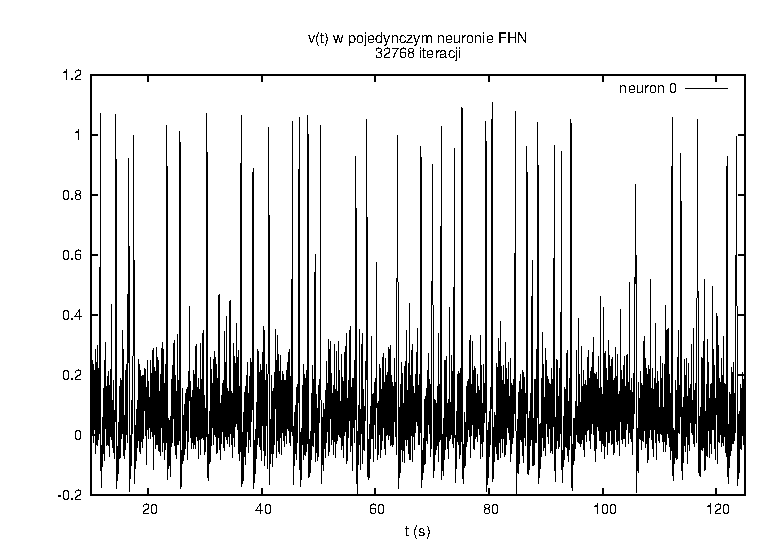
\includegraphics[width=140mm]{images/1neuron/1}} \\
        \resizebox{100mm}{!}{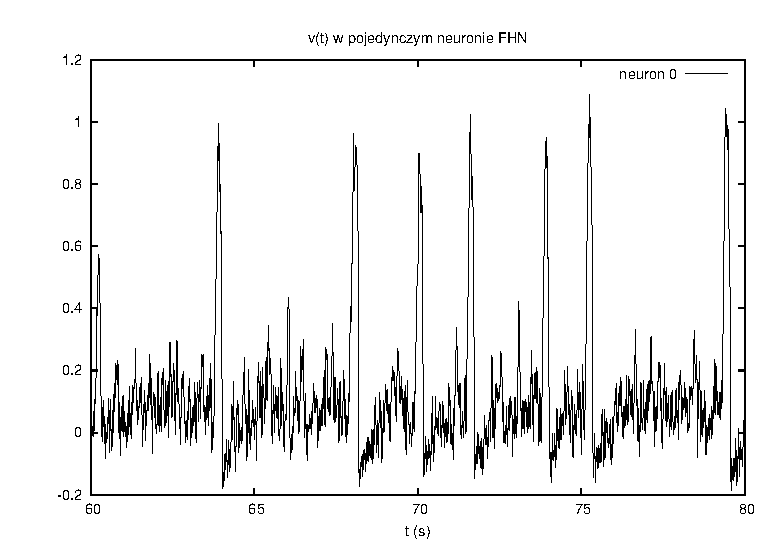
\includegraphics[width=140mm]{images/1neuron/2}} \\
      \end{tabular}
      \caption{Odtworzenie wyników Longtina (UZUPEŁNIĆ)}
      \label{sym1v}
    \end{center}
  \end{figure}

  Jest to przebieg zgodny z zaobserwowanym w pracy A. Longtin.

  \begin{figure}
    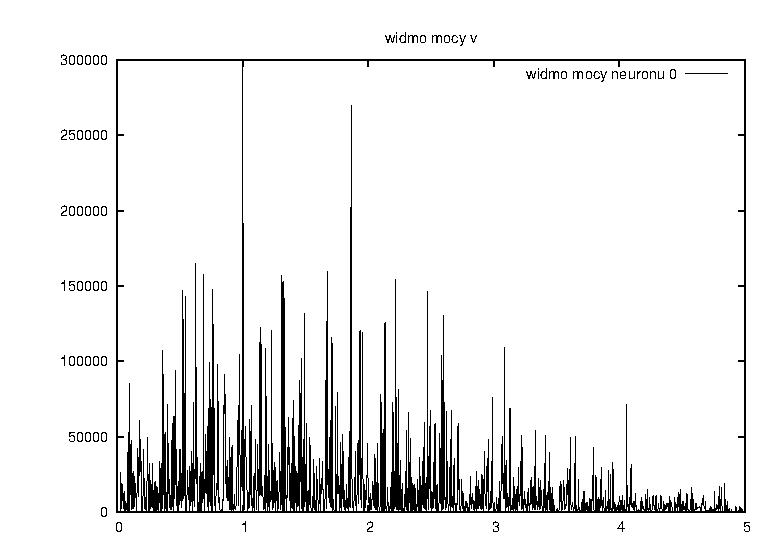
\includegraphics[width=140mm]{images/1neuron/3}
    \caption{FFT odtworzenie wyników longtina}
    \label{sym1fft}
  \end{figure}

  
  \subsection{Układy Neuronów Bez Opóźnienia}
  
  Następnym krokiem pracy było połączenie neuronów (początkowo dwóch) w ''sznur'', z sygnałem przekazywanym w jedną stronę, tzn. sygnał z neuronu i jest odbierany przez neuron i-1 (neuron o numerze 0 nie przekazuje swojego sygnału dalej). Neurony w układzie działały według równania zaproponowanego w rozdziale ~\ref{sec:przesuniecie_fazy}, bez opóźnienia (czyli $\tau_{n} = 0$)
  
  \begin{figure}
    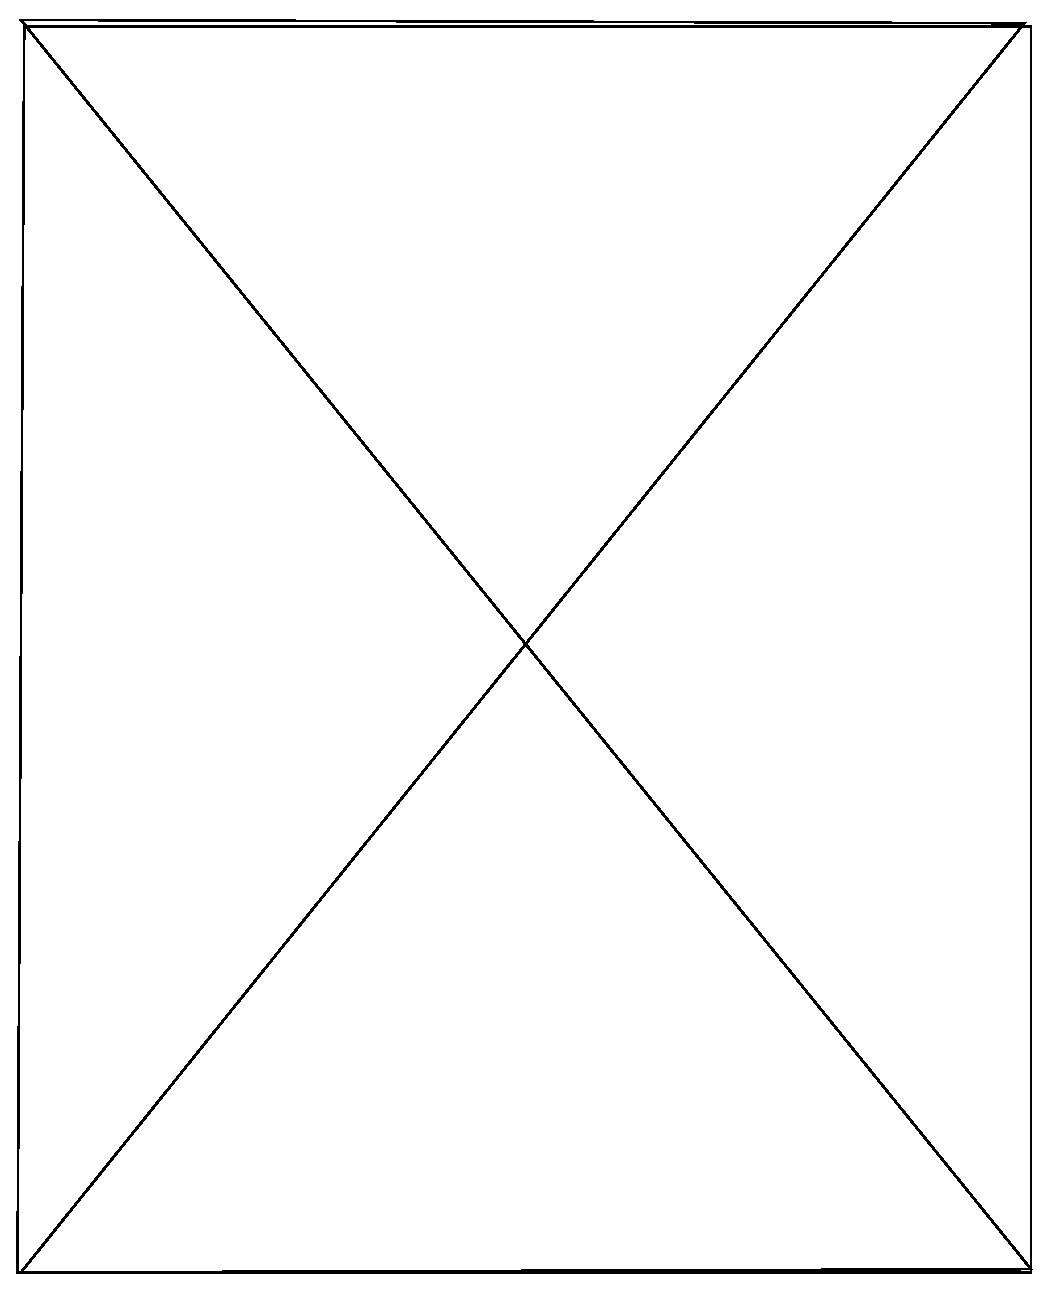
\includegraphics[width=120mm]{images/pending}
    \caption{Układ kilku (?) neuronów bez opóźnienia. Widać wyraźny wzrost SNR zgodnie z ''kierunkiem'' przekazywania sygnału.}
    \label{fig:graphics:sim:x}
  \end{figure}

  Zaobserwowane przebiegi czasowe były zgodne ze spodziewanym analitycznie wynikiem: z każdym kolejnym neuronem w łańcuchu następował wzrost SNR (DO WARTOŚCI GRANICZNEJ) ze względu na wzrost prawdopodobieństwa wzbudzenia w przypadku wzbudzenia neuronu sąsiedniego.


  
  \subsection{Układy Neuronów Z Opóźnieniem}
  
  Do układu opisanego powyżej dodałem opóźnienie w przekazywaniu sygnałów, w sposób opisany w rozdziale ~\ref{sec:przesuniecie_fazy}

  \begin{figure}
    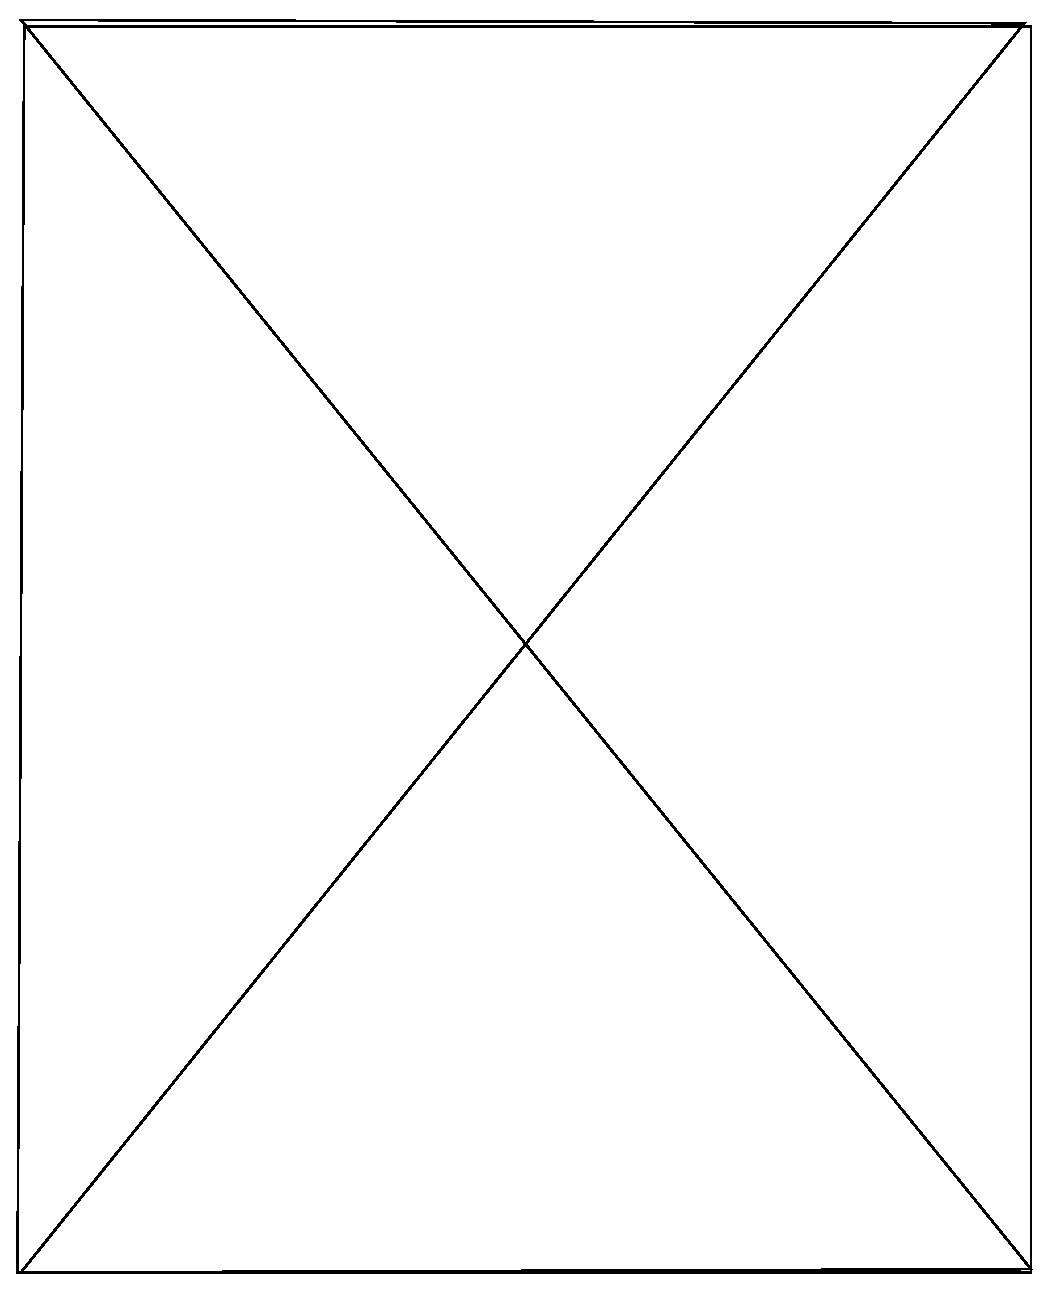
\includegraphics[width=120mm]{images/pending}
    \caption{Układ kilku (?) neuronów bez opóźnienia. Widać wyraźny wzrost SNR zgodnie z ''kierunkiem'' przekazywania sygnału.}
    \label{fig:graphics:sim:xx}
  \end{figure}
  
  
  \subsubsection{Macierz Dwóch Neuronów}

  Pierwszym krokiem w badaniu macierzy neuronów z opóźnieniem uczyniłem zbadanie macierzy dwuelementowej, celem znalezienia zależności pomiędzy podstawowymi parametrami symulacji.

  Przez c oznaczyłem opóźnienie transmisji, jako wielokrotność okresu sygnału periodycznego. Przesunięcie fazowe sygnału periodycznego p wynosiło pół okresu.
  Znaleziona zależność SNR (WYKRES) od c oraz D (skalowanie szumu) posiada bardzo wyraźną ''grań'' dla c=0.5, co potwierdza oczekiwania: maksymalizację SNR można osiągnąć poprzez kompensację przesunięcia fazowego (rozciągłości przestrzennej) identycznym (lub prawie identycznym) opóźnieniem w transmisji.

  \begin{figure}
    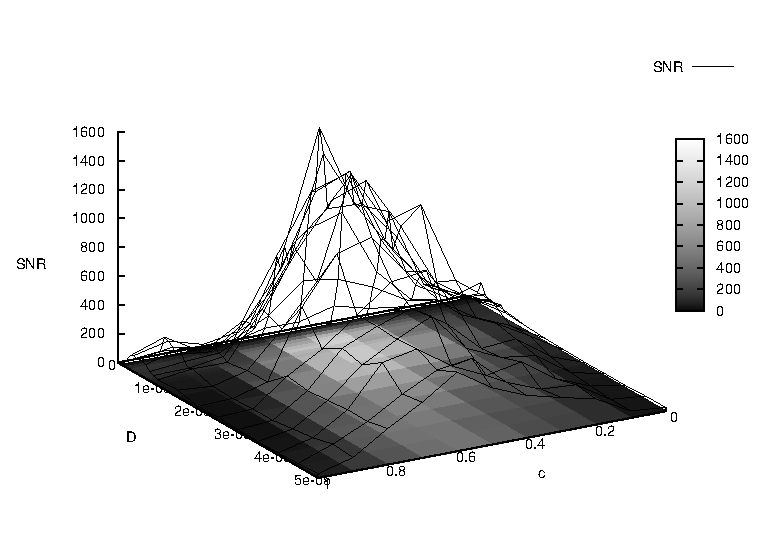
\includegraphics[width=140mm]{images/2neuron/3d}
    \caption{Dwa neurony, SNR w ''odbierającym'' w zależności od opóźnienia w transmisji c (jako wielokrotność T), dla przesunięcia fazowego równego 0.5T. Widać wyraźną ''grań'' kiedy c = p (= 0.5T)}
    \label{snr_c_d_3d}
  \end{figure}


